\chapter{Theoretical framework}

This chapter will cover the main theoretical topics addressed during the development of the thesis. 
The aim of this exposition is not to exhaustively cover the research conducted in the various fields 
but to provide a sufficient overview to undertake the experimentation carried out.

\section{Sentiment Analysis}

The task of Sentiment Analysis\cite{SentAnalysis} finds its theoretical framework in the broader context of Natural Language Processing (NLP). 
NLP refers to algorithmic techniques aimed at manipulating, extracting information from, or generally ``understanding'' written text.

This field of research has roots in the early days of computer science and has always held significant interest for researchers in artificial intelligence.

Currently, the majority of natural language processing techniques employ deep learning models, 
particularly models based on the attention mechanism known as Transformers\cite{Attention}.

Sentiment Analysis is no exception, and the most promising models today are based on BERT\cite{BERT}, 
a method for encoding textual information that uses a contextual vector representation. 
This approach allows for the dynamic analysis of words, making it easier to capture the differences in meaning due to their position in the text.

Specifically, the task of Sentiment Analysis aims to classify provided examples into two or more classes based on the sentiment conveyed in the sentence. 
The binary version of this classification mechanism involves dividing the input data based on whether they transmit a ``positive'' or ``negative'' emotion.

The success of this type of classification is crucial in contexts such as social networks\cite{SentTweeter}, 
where these tools can enhance the ability of algorithms to autonomously moderate published content, 
thus avoiding excessive use of hate speech. 
Another application context where Sentiment Analysis is fundamental for optimal success is machine translation. 
Some languages are naturally more prone to the use of irony, 
and if this nuance of meaning is not captured, a ``naive'' translation would result in a completely meaningless output.

\section{Support vector machine}

\note{Image \ref{fig:svm-margins} is extracted from Esposito's slides, can I use it?}

Among the various machine learning models for binary classification, support vector machines\cite{SVM} (SVMs) aim to separate examples by generalizing them as effectively as possible. The underlying idea is to select, among the candidate separation lines, the one that maximizes the distance between the elements of the two classes. Provided the training dataset is balanced, this procedure ensures better generalization properties for examples near the decision boundary that discriminates between positive and negative examples.

\begin{wrapfigure}{l}{0.45\textwidth}
    \centering
    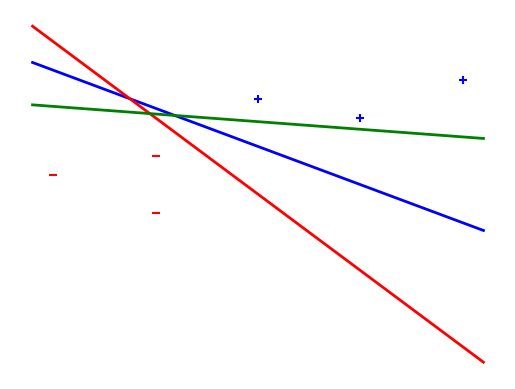
\includegraphics[width=0.4\textwidth]{figures/svm-intuition}
    \caption{Decision boundary.}
    \label{fig:svm-example}
\end{wrapfigure}

In Figure \ref{fig:svm-example}, we can visualize an example with two-dimensional data for classification. Among the different separation lines, it is intuitive to associate the blue one with the best generalization. This line not only correctly classifies all examples in the dataset but is also likely to generalize better during inference.

The formulation of SVMs is defined through a constraint satisfaction problem (CSP). To properly define the problem, it is necessary to introduce the notions of functional margin and geometric margin.

\paragraph{Functional Margin} The SVM model is described by a separating hyperplane represented by $f(x) = w \cdot x - t$. The functional margin is defined as $\mu(x) = y(w \cdot x - t) = yf(x)$. This function takes positive values if and only if the example is correctly classified. In the proposed formulation, $w$ and $t$ represent the model parameters to be derived during the learning phase. Intuitively, the functional margin indicates the rotation of the separation line in the example plane.

\paragraph{Geometric Margin} The geometric margin indicates the distance between the closest positive example to the decision boundary and the closest negative example. The formula to calculate its value is $\mu_g=(x_+-x_-)\cdot\frac{w}{||w||}$.

\begin{figure}[H]
    \centering
    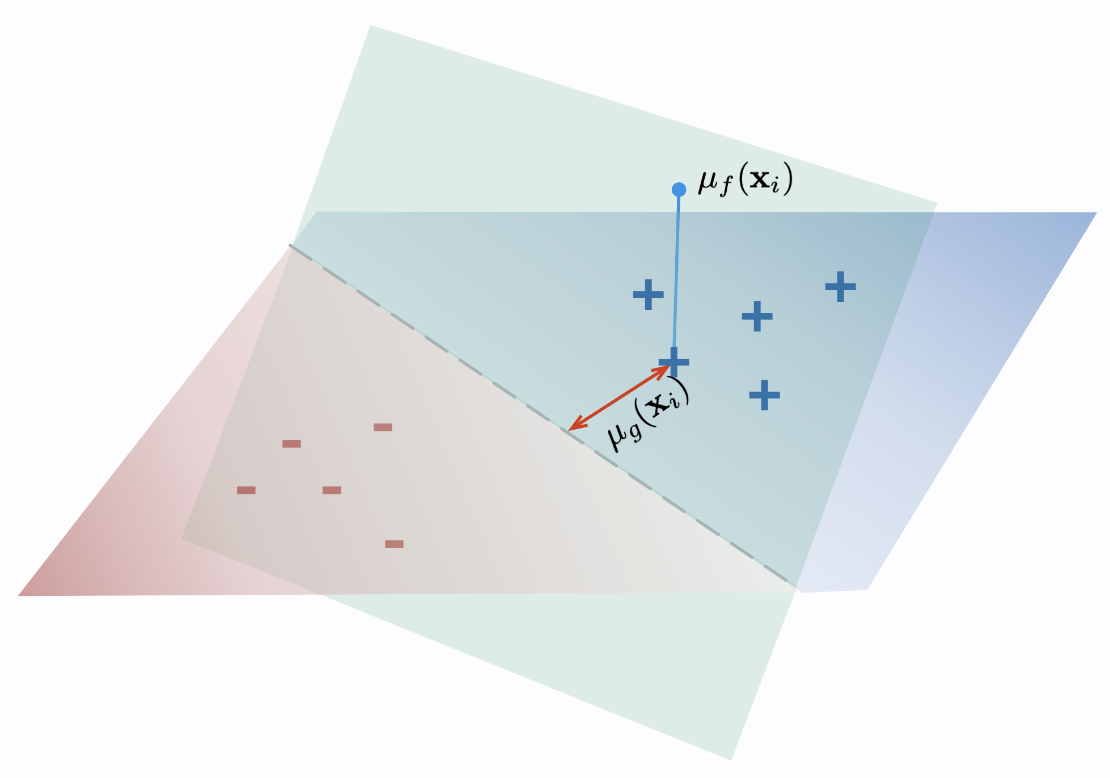
\includegraphics[width=0.7\textwidth]{figures/margins}
    \caption{Visual representation of the contribution of margins in defining the decision boundary.}
    \label{fig:svm-margins}
\end{figure}

\subsection{Primal Formulation}

The primal formulation of the optimization problem describing support vector machines takes the form:

\begin{align*}
    \min_{w, t}\ & \frac{1}{2}||w||^2 \\
    \text{subject to } & y_i(w \cdot x_i - 1)\geq 1 \quad \forall i:1\leq i\leq n
\end{align*}

In this case, the geometric margin is expressed in the objective function, while the functional margin is represented as a constraint of the problem.

\subsection{Derivation of the Dual Form}

The natural formulation for the problem, i.e., the primal, is not sufficiently efficient in terms of computation. However, its dual reformulation possesses some desirable properties. For instance, the dual problem depends only on the support vectors, i.e., the training dataset examples that lie on the margin.

The dual formulation for SVMs is derived starting from the Lagrangian relaxation.

$$\Lambda(w, t, \alpha) = \frac{1}{2}||w||^2 - \sum_{i=1}^n\alpha_i(y_i(w\cdot x_i - t) - 1)$$

This can be expanded into:

$$\frac{1}{2}w\cdot w - w\cdot\sum_{i=1}^n\alpha_iy_ix_i + t\sum_{i=1}^n\alpha_iy_i + \sum_{i=1}^n\alpha_i$$

To find the Lagrangian dual, we need to calculate the minimum of this function, which requires finding when the partial derivatives concerning $w$ and $t$ are zero.

$$\frac{\partial\Lambda}{\partial t} = \sum_{i=1}^n\alpha_iy_i = 0$$

$$\frac{\partial\Lambda}{\partial w} = w - \sum_{i=1}^n\alpha_iy_ix_i = 0 \to w = \sum_{i=1}^n\alpha_iy_ix_i$$

Substituting the results from the derivatives into the problem yields the dual formulation.

\begin{align*}
    \max_\alpha\ & -\frac{1}{2}\sum_{i=1}^n\sum_{j=1}^n\alpha_i\alpha_jy_iy_jx_ix_j + \sum_{i=1}^n
  \alpha_i \\
    \text{subject to } & 0 \leq \alpha_i \quad \forall i: 1\leq i\leq n \\
    & \sum_{i=1}^ny_i\alpha_i=0
\end{align*}

\subsubsection{Soft Margin}

The previously discussed problem does not allow for any error from the model, meaning that, in the case of non-linearly separable data, it will be impossible to find an optimal assignment for the CSP. This behavior is undesirable. To address this, the problem can be relaxed to accept the presence of errors.

Thus, the constraint of the functional margin in the primal problem is modified to $y_i(w\cdot x_i-t)\geq1-\xi_i$, while the objective function is augmented with the component $C\sum_{i=1}^n\xi_i$, where $C$ is a predefined parameter that indicates the penalty weight introduced by the errors.

Deriving the problem yields:

\begin{align*}
    \max_\alpha\ & -\frac{1}{2}\sum_{i=1}^n\sum_{j=1}^n\alpha_i\alpha_jy_iy_jx_ix_j + \sum_{i=1}^n
  \alpha_i \\
    \text{subject to } & 0 \leq \alpha_i \leq C \quad \forall i: 1\leq i\leq n \\
    & \sum_{i=1}^ny_i\alpha_i=0
\end{align*}

\subsubsection{Kernel Trick}

The introduction of the soft margin is not sufficient to handle most real-world problems. Simple datasets can be constructed where it is impossible to find a linear separation that does not produce a high error rate during inference.

A mapping function is introduced to project the dataset points into a higher-dimensional space.

\begin{theorem}[Cover]
  A pattern classification problem cast in a nonlinear high-dimensional space is more likely to be linearly separable than in a low-dimensional space\cite{ThCover}.
\end{theorem}

Instead of performing the multiplication $x_ix_j$, this multiplication can be substituted with $\langle\phi(x_i), \phi(x_j)\rangle$. For efficiency reasons, these inner product can be precomputed by generating the kernel matrix $K(x_i, x_j) = \langle\phi(x_i),\phi(x_j)\rangle$. Using kernel matrices allows the calculation of the result value without explicitly computing the mapping of each element. This difference, which might seem secondary at first glance, is fundamental as it allows the use of kernels that map to a potentially infinite-dimensional hyperspace.

Kernels can thus be used in the dual formulation of SVMs to generalize classification to datasets with non-linearly separable data.

\begin{align}
    \label{eq:svm-obj}
    \max_\alpha\ & -\frac{1}{2}\sum_{i=1}^n\sum_{j=1}^n\alpha_i\alpha_jy_iy_jK(x_i, x_j) + \sum_{i=1}^n\alpha_i \\ 
    \label{eq:svm-c1}
    \text{subject to } & 0 \leq \alpha_i \leq C \quad \forall i: 1\leq i\leq n \\
    \label{eq:svm-c2}
    & \sum_{i=1}^ny_i\alpha_i=0
\end{align}

\subsubsection{Inference with the Dual Solution}

Solving the problem using the dual formulation does not directly provide the values of $w$ and $t$. These values need to be derived to use the result in the inference phase.

The coefficient $t$ can be calculated as an average of the results obtained with the support vectors.

$$t = \frac{\sum_{i=1}^n y_i - \sum_{j=1}^n(\alpha_jy_jK(x_i,x_j))}{n}$$

As for the value of $w$, it cannot be directly derived when using the kernel function. The new $f(x)$ formulation becomes:

\begin{equation}
  f(x)=\sum_{i=1}^n\alpha_iy_iK(x_i, x) + t\label{eq:svm-predict}
\end{equation}

\section{Adiabatic quantum computing}

To overcome some of the limitations of classical computing, alternative architectures have been developed. Prominent among these is quantum computing, a branch of information theory that has achieved important milestones in recent years, enabling its application in real-world contexts.

The two paradigms currently in use when discussing quantum computing are the gate-based approach and the adiabatic approach.

\subsection{Gate-based quantum computing}

Gate-based quantum computing involves the direct manipulation of qubits using quantum gates\cite{QGate}. This low-level approach is analogous to working directly with logic gates in a classical architecture. Quantum gates (distinct from classical gates) enable the creation of true general-purpose computational models, capable of performing any type of calculation. The computational advantage arises from the use of quantum phenomena, such as entanglement, and the use of superposition to ``search'' for the solution to a problem by exploring multiple states simultaneously, collapsing the solution only at the moment of measurement.

IBM is a leading company in this field, currently operating quantum computers with a qubit count in the hundreds.

\begin{figure}[H]
  \centering
  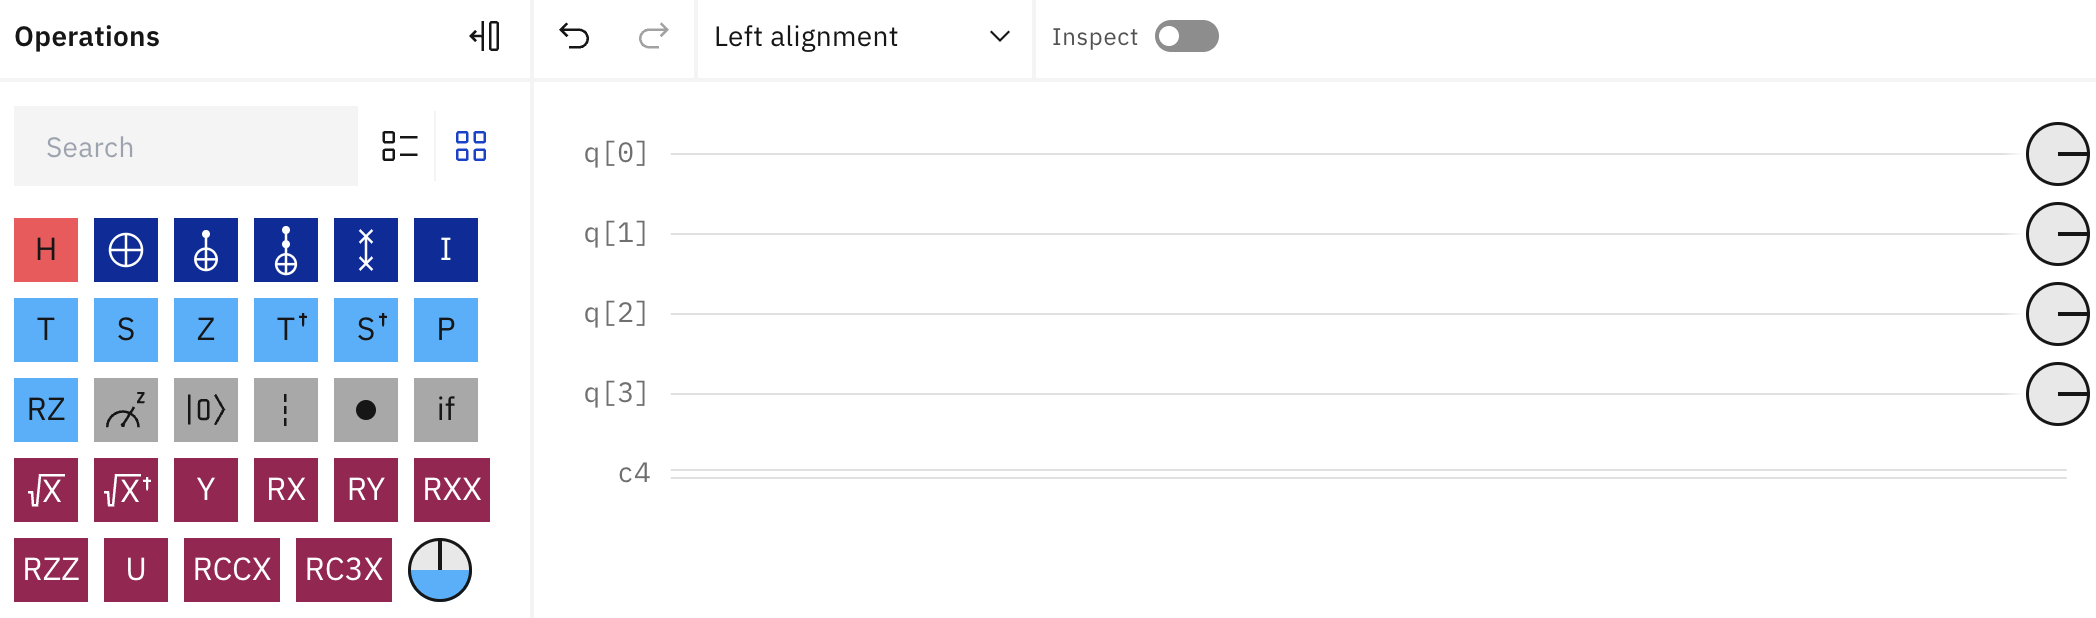
\includegraphics[width=\textwidth]{figures/4qubit}
  \caption{IBM quantum composer. Available gates and qubit system.}
\end{figure}

Although gate-based architecture represents a more generic computational model, the limitations due to the number of qubits and the error rates of these systems have led to the development of alternatives that can be used with the resources available. The most promising among these is adiabatic quantum computing.

\subsection{Adiabatic-based quantum computing}\label{sec:AQC}

Adiabatic quantum computing\cite{AQC} (AQC) is not aimed at creating a complete computational system. Instead, its goal is to exploit quantum phenomena to accelerate the optimization of models\cite{AQC2}. Specifically, D-Wave’s implementation of AQC follows these logical steps:

\begin{enumerate}
  \item Transform the problem into a Quadratic Unconstrained Binary Optimization (QUBO) formulation.
  \item Convert the objective function into a minimization problem.
  \item Generate the graph that represents the problem.
  \item Map this graph onto the qubit graph that forms the Quantum Processing Unit (QPU).
  \item Use quantum annealing to return the assignment that minimizes the objective function.
\end{enumerate}

This overview is a high-level representation of the steps required to utilize quantum annealing technologies. The complexity of the procedure is not immediately apparent at this level of abstraction, necessitating a detailed analysis of each step for a comprehensive understanding.

\paragraph{Minimization of Problems in QUBO Form} QUBO, an acronym for Quadratic Unconstrained Binary Optimization, is a standard formulation for expressing satisfaction problems. Specifically, all the information is encapsulated in the objective function, which takes the form $x^T Q x$, where $x$ is a column vector representing the optimization variables (with binary domain) and $Q$ is an upper triangular matrix describing the relationships between the variables. 

\begin{center} 
  $\underbrace{\begin{bmatrix}
      x_1 & \cdots & x_n 
  \end{bmatrix}}_{\bar{x}^T}$ 
  $\underbrace{\begin{bmatrix}
      a_1 & \cdots & a_n \\
      \vdots & \ddots & b_n \\
      0 & \cdots & c_n 
  \end{bmatrix}}_{Q}$ 
  $\underbrace{\begin{bmatrix}
      x_1 \\
      \vdots \\
      x_n 
  \end{bmatrix}}_{\bar{x}}$       
\end{center}

For use with adiabatic quantum computing, the QUBO problem must be in minimization form. Without loss of generality, any maximization problem can be transformed into a minimization problem, yielding the standard form for quantum machines: $\min x^T Q x$.

\paragraph{Problem graph for QUBO} The QPU does not directly manipulate QUBO problems but searches for the state with the lowest entropy (or energy) of a graph. The QUBO representation can be naturally rewritten into an undirected graph. The coefficients in the matrix $Q[i, j]$ represent the weight of the edge from node $i$ to node $j$. In the case of coefficients on the main diagonal, the edges enter and exit the same node.

For example, consider the following QUBO problem:

\begin{center} 
  $\begin{bmatrix}
    x_1 & x_2 & x_3 & x_4
  \end{bmatrix}$
  $\begin{bmatrix}
    -3 & 5 & 1 & -7 \\
    0 & 1 & 0 & 8 \\
    0 & 0 & 9 & -4 \\
    0 & 0 & 0 & -2 
  \end{bmatrix}$
  $\begin{bmatrix}
    x_1 \\ x_2 \\ x_3 \\ x_4
  \end{bmatrix}$      
\end{center}

Generates the following undirected graph:

\begin{figure}[H]
  \centering
  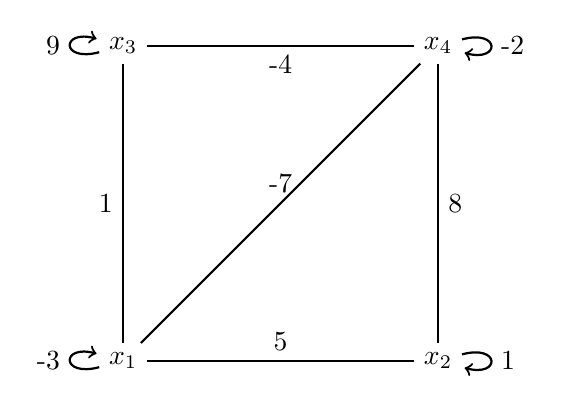
\begin{tikzpicture}
    \node (x1) at (0, 0) {$x_1$};
    \node (x2) at (4, 0) {$x_2$};
    \node (x3) at (0, 4) {$x_3$};
    \node (x4) at (4, 4) {$x_4$};

    \path[draw, thick] 
      (x1) edge[above] node{5} (x2)
      (x1) edge[left] node{1} (x3)
      (x1) edge[above] node{-7} (x4)
      (x2) edge[right] node{8} (x4)
      (x3) edge[below] node{-4} (x4);
  
    \path[draw, thick, looseness=10, out=135, in=225] 
      (x1) edge[loop left] node{-3} (x1)
      (x2) edge[loop right] node{1} (x2)
      (x3) edge[loop left] node{9} (x3)
      (x4) edge[loop right] node{-2} (x4);
  \end{tikzpicture}
  \caption{Graph of the proposed problem.}
  \label{fig:problem-graph}
\end{figure}

\paragraph{Minor graph embedding} As previously mentioned, the structure of the QPU\cite{Pegasus} is fixed, and this structure determines the number and connections between the Qubits.

Imagining a QPU with 32 Qubits, its shape would be approximately as follows:

\begin{figure}[H]
  \begin{center}
      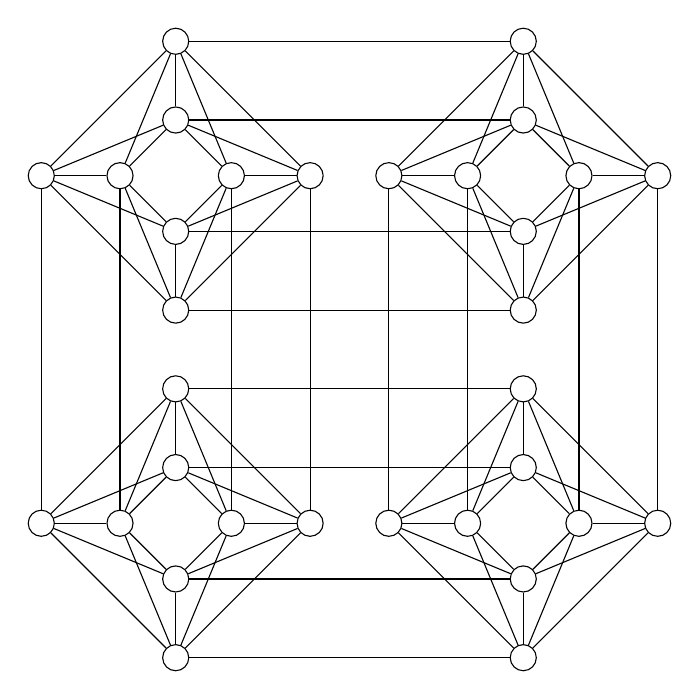
\begin{tikzpicture}[main/.style = {draw, circle}] 
          \node[main](1){};
          \node[main](2)[right of=1]{}; 
          \node[main](5)[above right of=2]{};
          \node[main](6)[above of=5]{};
          \node[main](3)[below right of=5]{};
          \node[main](4)[right of=3]{};
          \node[main](7)[below right of=2]{};
          \node[main](8)[below of=7]{};
  
          \draw (1) -- (6);\draw (6) -- (4);\draw (4) -- (8);\draw (8) -- (1);
          \draw (1) -- (5);\draw (5) -- (4);\draw (4) -- (7);\draw (7) -- (1);
          \draw (6) -- (2);\draw (2) -- (8);\draw (8) -- (3);\draw (3) -- (6);
          \draw (2) -- (5);\draw (5) -- (3);\draw (3) -- (7);\draw (7) -- (2);
          \draw (1) -- (2);\draw (5) -- (6);\draw (3) -- (4);\draw (8) -- (7);
  
          \node[main](11)[right of=4]{};
          \node[main](12)[right of=11]{}; 
          \node[main](15)[above right of=12]{};
          \node[main](16)[above of=15]{};
          \node[main](13)[below right of=15]{};
          \node[main](14)[right of=13]{};
          \node[main](17)[below right of=12]{};
          \node[main](18)[below of=17]{};
  
          \draw (11) -- (16);\draw (16) -- (14);\draw (14) -- (18);\draw (18) -- (11);
          \draw (11) -- (15);\draw (15) -- (14);\draw (14) -- (17);\draw (17) -- (11);
          \draw (16) -- (12);\draw (12) -- (18);\draw (18) -- (13);\draw (13) -- (16);
          \draw (12) -- (15);\draw (15) -- (13);\draw (13) -- (17);\draw (17) -- (12);
          \draw (11) -- (12);\draw (15) -- (16);\draw (13) -- (14);\draw (18) -- (17);
  
          \node[main](26)[below of=8]{};
          \node[main](25)[below of=26]{};
          \node[main](22)[below left of=25]{};
          \node[main](21)[left of=22]{};
          \node[main](23)[below right of=25]{};
          \node[main](24)[right of=23]{};
          \node[main](27)[below right of=22]{};
          \node[main](28)[below of=27]{};
  
          \draw (21) -- (26);\draw (26) -- (24);\draw (24) -- (28);\draw (28) -- (21);
          \draw (21) -- (25);\draw (25) -- (24);\draw (24) -- (27);\draw (27) -- (21);
          \draw (26) -- (22);\draw (22) -- (28);\draw (28) -- (23);\draw (23) -- (26);
          \draw (22) -- (25);\draw (25) -- (23);\draw (23) -- (27);\draw (27) -- (22);
          \draw (21) -- (22);\draw (25) -- (26);\draw (23) -- (24);\draw (28) -- (27);
  
          \node[main](36)[below of=18]{};
          \node[main](35)[below of=36]{};
          \node[main](32)[below left of=35]{};
          \node[main](31)[left of=32]{};
          \node[main](33)[below right of=35]{};
          \node[main](34)[right of=33]{};
          \node[main](37)[below right of=32]{};
          \node[main](38)[below of=37]{};
  
          \draw (31) -- (36);\draw (36) -- (34);\draw (34) -- (38);\draw (38) -- (31);
          \draw (31) -- (35);\draw (35) -- (34);\draw (34) -- (37);\draw (37) -- (31);
          \draw (36) -- (32);\draw (32) -- (38);\draw (38) -- (33);\draw (33) -- (36);
          \draw (32) -- (35);\draw (35) -- (33);\draw (33) -- (37);\draw (37) -- (32);
          \draw (31) -- (32);\draw (35) -- (36);\draw (33) -- (34);\draw (38) -- (37);
  
          \draw (6) -- (16);
          \draw (5) -- (15);
          \draw (7) -- (17);
          \draw (8) -- (18);
          \draw (26) -- (36);
          \draw (25) -- (35);
          \draw (27) -- (37);
          \draw (28) -- (38);
          \draw (1) -- (21);
          \draw (2) -- (22);
          \draw (3) -- (23);
          \draw (4) -- (24);
          \draw (11) -- (31);
          \draw (12) -- (32);
          \draw (13) -- (33);
          \draw (14) -- (34);
      \end{tikzpicture} 
      \caption{32 QuBit QPU.}
      \label{fig:QPU}
  \end{center}
\end{figure}

The structure of the Qubits is characterized by this ``diamond'' shape that D-Wave calls Pegasus. The currently available QPUs have approximately 5500 Qubits, in which a pattern similar to the one shown in figure \ref{fig:QPU} is repeated.

To embed the graph \ref{fig:problem-graph} into the QPU, the nodes must be arranged appropriately. Direct mapping is not always possible, and in such cases, the minor embedding procedure\cite{ME} is necessary. The minor embedding algorithm constructs chains of qubits that map multiple physical nodes of the QPU to the same logical node of the original graph. This approach compensates for the limited connections of the QPU and ensures all necessary nodes are connected.

A possible embedding for \ref{fig:problem-graph} might be:

\begin{figure}[H]
  \begin{center}
      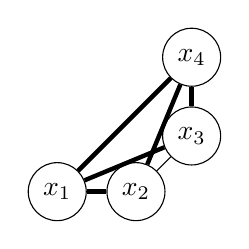
\begin{tikzpicture}[main/.style = {draw, circle}] 
          \node[main](1){$x_1$};
          \node[main](2)[right of=1]{$x_2$}; 
          \node[main](5)[above right of=2]{$x_3$};
          \node[main](6)[above of=5]{$x_4$};
  
          \draw[ultra thick] (1) -- (6); \draw[ultra thick] (1) -- (5); \draw[ultra thick] (6) -- (2); 
          \draw[ultra thick] (5) -- (6); \draw[ultra thick] (1) -- (2); \draw (2) -- (5);
      \end{tikzpicture} 
      \caption{Embedded problem}
      \label{fig:embedding}
  \end{center}
\end{figure}

\paragraph{Quantum annealing} 

Once the graph is mapped onto the QPU, the search for the assignment that minimizes the energy expressed by the physical system can begin. The two main phenomena during this process are annealing and quantum tunnelling.

The annealing phenomenon (referred to as thermal jump in figure \ref{fig:q-anneal}), which is also present in various local search techniques like simulated annealing\cite{SimulatedAnnealing}, aims to escape local minima. The idea behind this technique is to allow a state change that temporarily increases the total energy, with the hope that from this new state, a global minimum can be reached.

To further avoid local minima, quantum computing leverages the tunnelling phenomenon. The physical system can naturally change states towards a more stable configuration with lower energy. This physical process helps avoid searching by climbing peaks, thus accelerating convergence towards the global minimum.

\begin{figure}[H]
  \centering
  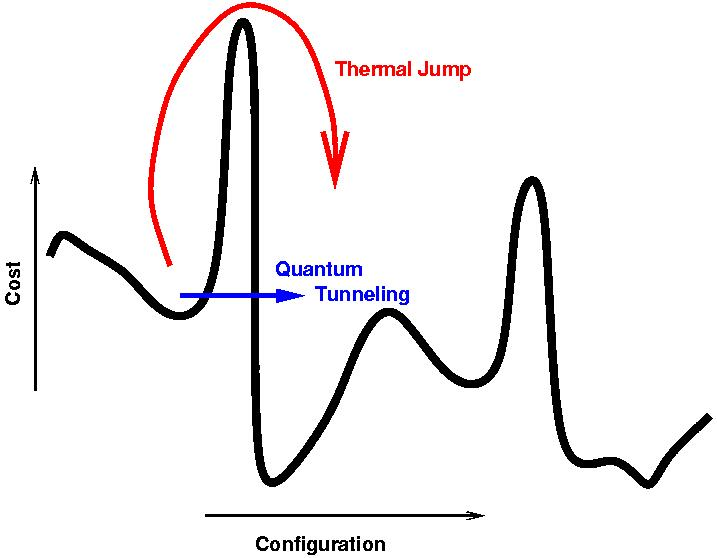
\includegraphics[width=0.5\textwidth]{figures/q-annealing.jpg}
  \caption{Graphical representation of quantum annealing.}
  \label{fig:q-anneal}
\end{figure}